\documentclass{standalone}
\usepackage{tikz}
\begin{document}
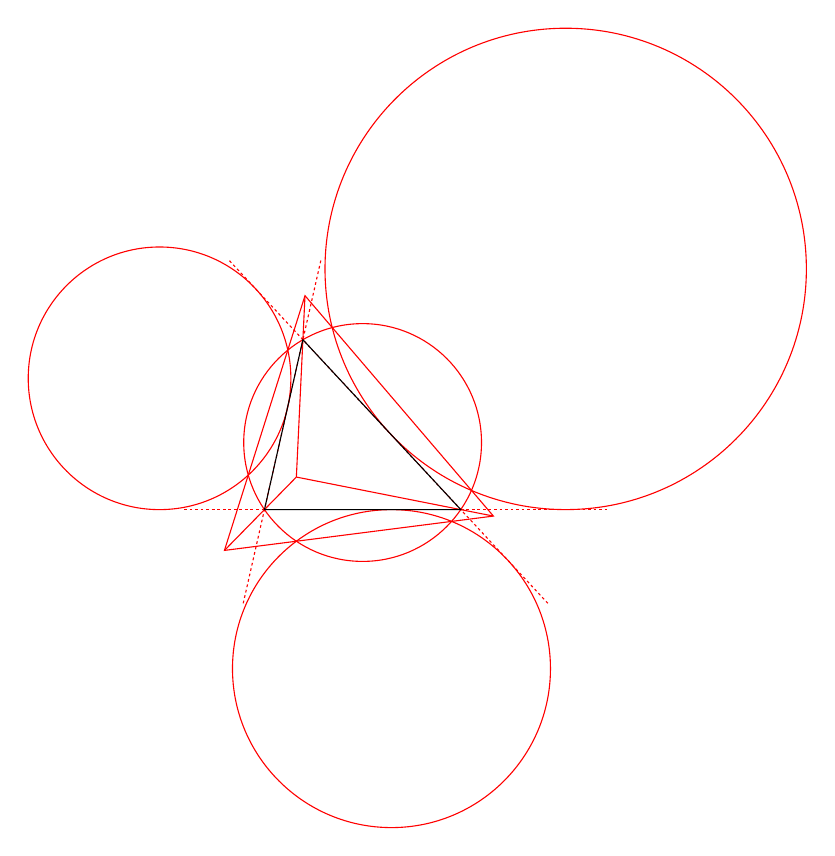
\begin{tikzpicture}[x=1pt,y=1pt]
\draw[red] (51.43,-130.73) circle (47.45);
\draw[red] (198.19,-91.20) circle (86.97);
\draw[red] (135.24,-235.63) circle (57.45);
\draw[red] (124.81,-153.93) circle (42.96);
\draw[red, dash pattern=on 1pt] (81.67,-212.04) -- (109.78,-87.85);
\draw[red, dash pattern=on 1pt] (191.75,-212.04) -- (76.35,-87.85);
\draw[red, dash pattern=on 1pt] (60.29,-178.17) -- (213.05,-178.17);
\draw[red] (100.87,-166.41) -- (103.98,-101.00);
\draw[red] (100.87,-166.41) -- (75.00,-192.80);
\draw[red] (100.87,-166.41) -- (171.86,-180.47);
\draw (160.28,-178.17) -- (103.23,-116.78) -- (89.34,-178.17) -- cycle;
\draw[red] (103.99,-100.87) -- (74.88,-192.92) -- (172.07,-180.51) -- cycle;
\end{tikzpicture}
\end{document}
